\documentclass[]{book}
\usepackage{lmodern}
\usepackage{amssymb,amsmath}
\usepackage{ifxetex,ifluatex}
\usepackage{fixltx2e} % provides \textsubscript
\ifnum 0\ifxetex 1\fi\ifluatex 1\fi=0 % if pdftex
  \usepackage[T1]{fontenc}
  \usepackage[utf8]{inputenc}
\else % if luatex or xelatex
  \ifxetex
    \usepackage{mathspec}
  \else
    \usepackage{fontspec}
  \fi
  \defaultfontfeatures{Ligatures=TeX,Scale=MatchLowercase}
\fi
% use upquote if available, for straight quotes in verbatim environments
\IfFileExists{upquote.sty}{\usepackage{upquote}}{}
% use microtype if available
\IfFileExists{microtype.sty}{%
\usepackage{microtype}
\UseMicrotypeSet[protrusion]{basicmath} % disable protrusion for tt fonts
}{}
\usepackage{hyperref}
\hypersetup{unicode=true,
            pdftitle={A Minimal Book Example},
            pdfauthor={Yihui Xie},
            pdfborder={0 0 0},
            breaklinks=true}
\urlstyle{same}  % don't use monospace font for urls
\usepackage{natbib}
\bibliographystyle{apalike}
\usepackage{color}
\usepackage{fancyvrb}
\newcommand{\VerbBar}{|}
\newcommand{\VERB}{\Verb[commandchars=\\\{\}]}
\DefineVerbatimEnvironment{Highlighting}{Verbatim}{commandchars=\\\{\}}
% Add ',fontsize=\small' for more characters per line
\usepackage{framed}
\definecolor{shadecolor}{RGB}{248,248,248}
\newenvironment{Shaded}{\begin{snugshade}}{\end{snugshade}}
\newcommand{\AlertTok}[1]{\textcolor[rgb]{0.94,0.16,0.16}{#1}}
\newcommand{\AnnotationTok}[1]{\textcolor[rgb]{0.56,0.35,0.01}{\textbf{\textit{#1}}}}
\newcommand{\AttributeTok}[1]{\textcolor[rgb]{0.77,0.63,0.00}{#1}}
\newcommand{\BaseNTok}[1]{\textcolor[rgb]{0.00,0.00,0.81}{#1}}
\newcommand{\BuiltInTok}[1]{#1}
\newcommand{\CharTok}[1]{\textcolor[rgb]{0.31,0.60,0.02}{#1}}
\newcommand{\CommentTok}[1]{\textcolor[rgb]{0.56,0.35,0.01}{\textit{#1}}}
\newcommand{\CommentVarTok}[1]{\textcolor[rgb]{0.56,0.35,0.01}{\textbf{\textit{#1}}}}
\newcommand{\ConstantTok}[1]{\textcolor[rgb]{0.00,0.00,0.00}{#1}}
\newcommand{\ControlFlowTok}[1]{\textcolor[rgb]{0.13,0.29,0.53}{\textbf{#1}}}
\newcommand{\DataTypeTok}[1]{\textcolor[rgb]{0.13,0.29,0.53}{#1}}
\newcommand{\DecValTok}[1]{\textcolor[rgb]{0.00,0.00,0.81}{#1}}
\newcommand{\DocumentationTok}[1]{\textcolor[rgb]{0.56,0.35,0.01}{\textbf{\textit{#1}}}}
\newcommand{\ErrorTok}[1]{\textcolor[rgb]{0.64,0.00,0.00}{\textbf{#1}}}
\newcommand{\ExtensionTok}[1]{#1}
\newcommand{\FloatTok}[1]{\textcolor[rgb]{0.00,0.00,0.81}{#1}}
\newcommand{\FunctionTok}[1]{\textcolor[rgb]{0.00,0.00,0.00}{#1}}
\newcommand{\ImportTok}[1]{#1}
\newcommand{\InformationTok}[1]{\textcolor[rgb]{0.56,0.35,0.01}{\textbf{\textit{#1}}}}
\newcommand{\KeywordTok}[1]{\textcolor[rgb]{0.13,0.29,0.53}{\textbf{#1}}}
\newcommand{\NormalTok}[1]{#1}
\newcommand{\OperatorTok}[1]{\textcolor[rgb]{0.81,0.36,0.00}{\textbf{#1}}}
\newcommand{\OtherTok}[1]{\textcolor[rgb]{0.56,0.35,0.01}{#1}}
\newcommand{\PreprocessorTok}[1]{\textcolor[rgb]{0.56,0.35,0.01}{\textit{#1}}}
\newcommand{\RegionMarkerTok}[1]{#1}
\newcommand{\SpecialCharTok}[1]{\textcolor[rgb]{0.00,0.00,0.00}{#1}}
\newcommand{\SpecialStringTok}[1]{\textcolor[rgb]{0.31,0.60,0.02}{#1}}
\newcommand{\StringTok}[1]{\textcolor[rgb]{0.31,0.60,0.02}{#1}}
\newcommand{\VariableTok}[1]{\textcolor[rgb]{0.00,0.00,0.00}{#1}}
\newcommand{\VerbatimStringTok}[1]{\textcolor[rgb]{0.31,0.60,0.02}{#1}}
\newcommand{\WarningTok}[1]{\textcolor[rgb]{0.56,0.35,0.01}{\textbf{\textit{#1}}}}
\usepackage{longtable,booktabs}
\usepackage{graphicx,grffile}
\makeatletter
\def\maxwidth{\ifdim\Gin@nat@width>\linewidth\linewidth\else\Gin@nat@width\fi}
\def\maxheight{\ifdim\Gin@nat@height>\textheight\textheight\else\Gin@nat@height\fi}
\makeatother
% Scale images if necessary, so that they will not overflow the page
% margins by default, and it is still possible to overwrite the defaults
% using explicit options in \includegraphics[width, height, ...]{}
\setkeys{Gin}{width=\maxwidth,height=\maxheight,keepaspectratio}
\IfFileExists{parskip.sty}{%
\usepackage{parskip}
}{% else
\setlength{\parindent}{0pt}
\setlength{\parskip}{6pt plus 2pt minus 1pt}
}
\setlength{\emergencystretch}{3em}  % prevent overfull lines
\providecommand{\tightlist}{%
  \setlength{\itemsep}{0pt}\setlength{\parskip}{0pt}}
\setcounter{secnumdepth}{5}
% Redefines (sub)paragraphs to behave more like sections
\ifx\paragraph\undefined\else
\let\oldparagraph\paragraph
\renewcommand{\paragraph}[1]{\oldparagraph{#1}\mbox{}}
\fi
\ifx\subparagraph\undefined\else
\let\oldsubparagraph\subparagraph
\renewcommand{\subparagraph}[1]{\oldsubparagraph{#1}\mbox{}}
\fi

%%% Use protect on footnotes to avoid problems with footnotes in titles
\let\rmarkdownfootnote\footnote%
\def\footnote{\protect\rmarkdownfootnote}

%%% Change title format to be more compact
\usepackage{titling}

% Create subtitle command for use in maketitle
\providecommand{\subtitle}[1]{
  \posttitle{
    \begin{center}\large#1\end{center}
    }
}

\setlength{\droptitle}{-2em}

  \title{A Minimal Book Example}
    \pretitle{\vspace{\droptitle}\centering\huge}
  \posttitle{\par}
    \author{Yihui Xie}
    \preauthor{\centering\large\emph}
  \postauthor{\par}
      \predate{\centering\large\emph}
  \postdate{\par}
    \date{2019-08-15}

\usepackage{booktabs}

\begin{document}
\maketitle

{
\setcounter{tocdepth}{1}
\tableofcontents
}
\hypertarget{prerequisites}{%
\chapter{Prerequisites}\label{prerequisites}}

This is a \emph{sample} book written in \textbf{Markdown}. You can use anything that Pandoc's Markdown supports, e.g., a math equation \(a^2 + b^2 = c^2\).

The \textbf{bookdown} package can be installed from CRAN or Github:

\begin{Shaded}
\begin{Highlighting}[]
\KeywordTok{install.packages}\NormalTok{(}\StringTok{"bookdown"}\NormalTok{)}
\CommentTok{# or the development version}
\CommentTok{# devtools::install_github("rstudio/bookdown")}
\end{Highlighting}
\end{Shaded}

Remember each Rmd file contains one and only one chapter, and a chapter is defined by the first-level heading \texttt{\#}.

To compile this example to PDF, you need XeLaTeX. You are recommended to install TinyTeX (which includes XeLaTeX): \url{https://yihui.name/tinytex/}.

\hypertarget{introduction-to-r}{%
\chapter{Introduction to R}\label{introduction-to-r}}

This is a document with information from the Slides in the introduction to R workshop held at Tele2 during autumn 2019.

\hypertarget{module-1---introduction-to-r}{%
\chapter{Module 1 - introduction to R}\label{module-1---introduction-to-r}}

In it's simplest form R can be used as a calculator with \texttt{+}, \texttt{-}, \texttt{/} or \texttt{*}.

\begin{Shaded}
\begin{Highlighting}[]
\DecValTok{100} \OperatorTok{+}\StringTok{ }\DecValTok{4}
\end{Highlighting}
\end{Shaded}

\begin{verbatim}
## [1] 104
\end{verbatim}

Or

\begin{Shaded}
\begin{Highlighting}[]
\DecValTok{4} \OperatorTok{*}\StringTok{ }\DecValTok{6} \OperatorTok{-}\StringTok{ }\DecValTok{2}
\end{Highlighting}
\end{Shaded}

\begin{verbatim}
## [1] 22
\end{verbatim}

\begin{itemize}
\item
\end{itemize}

Create objects with \texttt{\textless{}-}, which is called \emph{the assign operator}.

\begin{Shaded}
\begin{Highlighting}[]
\NormalTok{x <-}\StringTok{ }\DecValTok{100} \OperatorTok{+}\StringTok{ }\DecValTok{4}
\NormalTok{x}
\end{Highlighting}
\end{Shaded}

\begin{verbatim}
## [1] 104
\end{verbatim}

\begin{itemize}
\item
\end{itemize}

The \emph{assign operater} \texttt{\textless{}-} can be reversed \texttt{-\textgreater{}}

\begin{Shaded}
\begin{Highlighting}[]
\DecValTok{100} \OperatorTok{+}\StringTok{ }\DecValTok{4}\NormalTok{ ->}\StringTok{ }\NormalTok{x}
\NormalTok{x}
\end{Highlighting}
\end{Shaded}

\begin{verbatim}
## [1] 104
\end{verbatim}

\begin{itemize}
\item
\end{itemize}

You can combine values, or objects in a new object with the function \texttt{c()} (\emph{c} for \emph{combine}).
When objects are combined they are called a \emph{vector}.

\begin{Shaded}
\begin{Highlighting}[]
\NormalTok{x <-}\StringTok{ }\KeywordTok{c}\NormalTok{(}\DecValTok{4}\NormalTok{, }\DecValTok{100} \OperatorTok{+}\StringTok{ }\DecValTok{4}\NormalTok{, }\DecValTok{10} \OperatorTok{*}\StringTok{ }\DecValTok{2}\NormalTok{)}
\NormalTok{x}
\end{Highlighting}
\end{Shaded}

\begin{verbatim}
## [1]   4 104  20
\end{verbatim}

Objects and vectors are not restrained to numerical values, you can use text in them as well.

\begin{Shaded}
\begin{Highlighting}[]
\NormalTok{text <-}\StringTok{ }\KeywordTok{c}\NormalTok{(}\StringTok{"hej"}\NormalTok{, }\StringTok{"jag"}\NormalTok{, }\StringTok{"älskar"}\NormalTok{, }\StringTok{"r"}\NormalTok{)}
\NormalTok{text}
\end{Highlighting}
\end{Shaded}

\begin{verbatim}
## [1] "hej"    "jag"    "älskar" "r"
\end{verbatim}

However, you cannot mix numerical and text values.

\begin{Shaded}
\begin{Highlighting}[]
\NormalTok{blandat <-}\StringTok{ }\KeywordTok{c}\NormalTok{(}\DecValTok{1}\NormalTok{, }\DecValTok{5}\NormalTok{, }\StringTok{"hej"}\NormalTok{, }\DecValTok{6}\NormalTok{)}
\NormalTok{blandat}
\end{Highlighting}
\end{Shaded}

\begin{verbatim}
## [1] "1"   "5"   "hej" "6"
\end{verbatim}

\hypertarget{missing-values}{%
\section{Missing values}\label{missing-values}}

\texttt{NA} is not \emph{zero}. It is not a value.

\begin{Shaded}
\begin{Highlighting}[]
\NormalTok{x <-}\StringTok{ }\KeywordTok{c}\NormalTok{(}\DecValTok{4}\NormalTok{, }\OtherTok{NA}\NormalTok{, }\DecValTok{2}\NormalTok{, }\DecValTok{50}\NormalTok{)}
\end{Highlighting}
\end{Shaded}

If check which values that are larger than two:

\begin{Shaded}
\begin{Highlighting}[]
\NormalTok{x }\OperatorTok{>}\StringTok{ }\DecValTok{2} 
\end{Highlighting}
\end{Shaded}

\begin{verbatim}
## [1]  TRUE    NA FALSE  TRUE
\end{verbatim}

Let's filter out all the \texttt{NA}'s:

\begin{Shaded}
\begin{Highlighting}[]
\NormalTok{x }\OperatorTok{==}\StringTok{ }\OtherTok{NA}
\end{Highlighting}
\end{Shaded}

\begin{verbatim}
## [1] NA NA NA NA
\end{verbatim}

Confusing?

\begin{Shaded}
\begin{Highlighting}[]
\NormalTok{fredriks_age <-}\StringTok{ }\OtherTok{NA}
\NormalTok{markus_age <-}\StringTok{ }\OtherTok{NA}
\NormalTok{fredriks_age }\OperatorTok{==}\StringTok{ }\NormalTok{markus_age}
\end{Highlighting}
\end{Shaded}

\begin{verbatim}
## [1] NA
\end{verbatim}

If we want to find an \texttt{NA} or filter out \texttt{NA}s we us \texttt{is.na()} instead.

\begin{Shaded}
\begin{Highlighting}[]
\KeywordTok{is.na}\NormalTok{(x)}
\end{Highlighting}
\end{Shaded}

\begin{verbatim}
## [1] FALSE  TRUE FALSE FALSE
\end{verbatim}

\texttt{na.rm} is a common argument in functions.

\begin{Shaded}
\begin{Highlighting}[]
\KeywordTok{mean}\NormalTok{(x)}
\end{Highlighting}
\end{Shaded}

\begin{verbatim}
## [1] NA
\end{verbatim}

We use \texttt{na.rm\ =\ TRUE}

\begin{Shaded}
\begin{Highlighting}[]
\KeywordTok{mean}\NormalTok{(x, }\DataTypeTok{na.rm =} \OtherTok{TRUE}\NormalTok{)}
\end{Highlighting}
\end{Shaded}

\begin{verbatim}
## [1] 18.66667
\end{verbatim}

\hypertarget{r-is-a-functional-programming-languange}{%
\section{R is a functional programming languange}\label{r-is-a-functional-programming-languange}}

\begin{itemize}
\tightlist
\item
  Functions reside in packages
\item
  Functional programming is great for Data Science
\end{itemize}

\hypertarget{functions}{%
\section{Functions}\label{functions}}

Just like in Excel

\begin{itemize}
\tightlist
\item
  mean()
\item
  median()
\item
  sd()
\item
  \ldots{}and so on
\end{itemize}

And mathematical

\begin{itemize}
\tightlist
\item
  log()
\item
  sin()
\item
  cos()
\item
  \ldots{}osv
\end{itemize}

\hypertarget{documentation}{%
\section{Documentation}\label{documentation}}

To access documentation about functions, i.e.~how they work, you just add a question mark in front of the function that you are interested in.

\begin{Shaded}
\begin{Highlighting}[]
\NormalTok{?}\KeywordTok{mean}\NormalTok{()}
\end{Highlighting}
\end{Shaded}

\hypertarget{excercices}{%
\section{Excercices}\label{excercices}}

\begin{itemize}
\tightlist
\item
  Use some of R's statistical functions on a numerical vector
\end{itemize}

\hypertarget{data.frame}{%
\section{data.frame}\label{data.frame}}

data.frames are a common format when doing data science in R. A data.frame is a rectangular table with one or more columns.

\begin{verbatim}
## # A tibble: 6 x 19
##    year month   day dep_time sched_dep_time dep_delay arr_time
##   <int> <int> <int>    <int>          <int>     <dbl>    <int>
## 1  2013     1     1      517            515         2      830
## 2  2013     1     1      533            529         4      850
## 3  2013     1     1      542            540         2      923
## 4  2013     1     1      544            545        -1     1004
## 5  2013     1     1      554            600        -6      812
## 6  2013     1     1      554            558        -4      740
## # ... with 12 more variables: sched_arr_time <int>, arr_delay <dbl>,
## #   carrier <chr>, flight <int>, tailnum <chr>, origin <chr>, dest <chr>,
## #   air_time <dbl>, distance <dbl>, hour <dbl>, minute <dbl>,
## #   time_hour <dttm>
\end{verbatim}

We can create our own data frames in R.

\begin{Shaded}
\begin{Highlighting}[]
\KeywordTok{data.frame}\NormalTok{(}\DataTypeTok{random_number =} \KeywordTok{rnorm}\NormalTok{(}\DecValTok{5}\NormalTok{))}
\end{Highlighting}
\end{Shaded}

\begin{verbatim}
##   random_number
## 1     1.1915942
## 2     0.5884946
## 3     0.1172920
## 4     1.0749540
## 5     0.3227870
\end{verbatim}

If you have two vectors of the same lenght you can combine them to a data.frame.

\begin{Shaded}
\begin{Highlighting}[]
\NormalTok{siffror <-}\StringTok{ }\KeywordTok{c}\NormalTok{(}\DecValTok{5}\NormalTok{,}\DecValTok{1}\NormalTok{,}\DecValTok{2}\NormalTok{,}\DecValTok{5}\NormalTok{)}
\NormalTok{ord <-}\StringTok{ }\KeywordTok{c}\NormalTok{(}\StringTok{"vad"}\NormalTok{, }\StringTok{"var"}\NormalTok{, }\StringTok{"det"}\NormalTok{, }\StringTok{"där"}\NormalTok{)}

\KeywordTok{data.frame}\NormalTok{(siffror, ord)}
\end{Highlighting}
\end{Shaded}

\begin{verbatim}
##   siffror ord
## 1       5 vad
## 2       1 var
## 3       2 det
## 4       5 där
\end{verbatim}

\hypertarget{packages}{%
\section{Packages}\label{packages}}

\begin{itemize}
\item
  To install a package from \texttt{CRAN} you use the function \texttt{install.packages("package")}.
\item
  After downloading a package your need to load it with \texttt{library(package)}.
\end{itemize}

\hypertarget{excercise}{%
\section{Excercise}\label{excercise}}

The package \texttt{tidyverse} is downloaded for you. Load it with \texttt{library()}.

\hypertarget{tidyverse-and-friends}{%
\section{tidyverse and friends}\label{tidyverse-and-friends}}

\begin{itemize}
\item
  tidyverse is a collection of packages for common tasks in data analysis.
\item
  They share a common philosophy
\item
  Easy to use
\item
  We will focus on tidyverse
\end{itemize}

\hypertarget{workflow-in-r}{%
\subsection{Workflow in R}\label{workflow-in-r}}

\begin{itemize}
\tightlist
\item
  Use projects
\item
  Never save your workspace
\end{itemize}

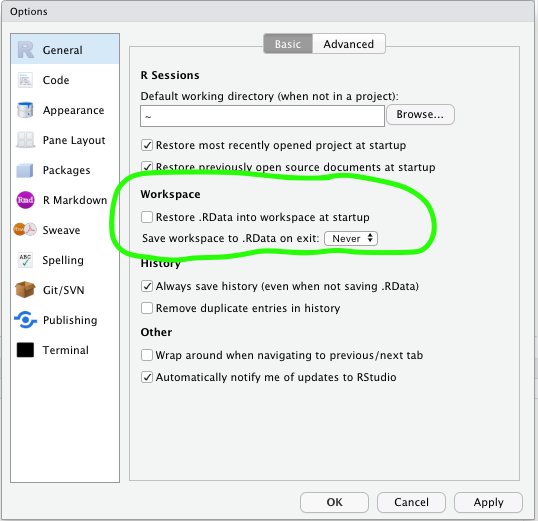
\includegraphics{_bookdown_files/presentation-intro_files/figure-html/workspace.png}

\hypertarget{writing-code-in-r}{%
\subsection{Writing code in R}\label{writing-code-in-r}}

\begin{itemize}
\tightlist
\item
  Follow the \texttt{tidyverse\ styleguide}
\end{itemize}

Name objects, functions and data.frames with \emph{small letters} and *\_* between words.

\begin{Shaded}
\begin{Highlighting}[]
\NormalTok{min_egna_funktion <-}\StringTok{ }\ControlFlowTok{function}\NormalTok{(x)}
\end{Highlighting}
\end{Shaded}

In contrast to:

\begin{Shaded}
\begin{Highlighting}[]
\NormalTok{MinEgnaFunktion <-}\StringTok{ }\ControlFlowTok{function}\NormalTok{(x)}
\end{Highlighting}
\end{Shaded}

\begin{itemize}
\tightlist
\item
  You are writing text for someone to read it
\item
  Use space between \texttt{,}
\end{itemize}

GOOD:

\begin{Shaded}
\begin{Highlighting}[]
\KeywordTok{mean}\NormalTok{(x, }\DataTypeTok{na.rm =} \OtherTok{TRUE}\NormalTok{)}
\end{Highlighting}
\end{Shaded}

BAD:

\begin{Shaded}
\begin{Highlighting}[]
\KeywordTok{mean}\NormalTok{(x,}\DataTypeTok{na.rm=}\OtherTok{TRUE}\NormalTok{)}
\end{Highlighting}
\end{Shaded}

\hypertarget{when-saving-files}{%
\section{When saving files}\label{when-saving-files}}

When saving files we try to follow this principle, so when you name a file name it \texttt{min\_r\_fil.R} instead of \texttt{min\ R\ fil.R}.

\hypertarget{avoid-long-expressions}{%
\section{Avoid long expressions}\label{avoid-long-expressions}}

This is harder to read:

\begin{Shaded}
\begin{Highlighting}[]
\NormalTok{iris }\OperatorTok\StringTok{ }\KeywordTok{group_by}\NormalTok{(Species) }\OperatorTok\StringTok{ }\KeywordTok{summarise}\NormalTok{(}\DataTypeTok{Sepal.Length =} \KeywordTok{mean}\NormalTok{(Sepal.Length), }\DataTypeTok{Sepal.Width =} \KeywordTok{mean}\NormalTok{(Sepal.Width), }\DataTypeTok{Species =} \KeywordTok{n_distinct}\NormalTok{(Species))}
\end{Highlighting}
\end{Shaded}

Than this:

\begin{Shaded}
\begin{Highlighting}[]
\NormalTok{iris }\OperatorTok
\StringTok{  }\KeywordTok{group_by}\NormalTok{(Species) }\OperatorTok
\StringTok{  }\KeywordTok{summarise}\NormalTok{(}
    \DataTypeTok{Sepal.Length =} \KeywordTok{mean}\NormalTok{(Sepal.Length),}
    \DataTypeTok{Sepal.Width =} \KeywordTok{mean}\NormalTok{(Sepal.Width),}
    \DataTypeTok{Species =} \KeywordTok{n_distinct}\NormalTok{(Species)}
\NormalTok{  ) }
\end{Highlighting}
\end{Shaded}

\hypertarget{rmarkdown}{%
\subsection{Rmarkdown}\label{rmarkdown}}

\begin{itemize}
\item
  A notebook format in R
\item
  Great for creating reports
\item
  Great for exploratory analysis
\item
  Open up \texttt{intro-to-r.Rmd}
\end{itemize}

\hypertarget{data-manipulation-with-dplyr}{%
\chapter{Data manipulation with dplyr}\label{data-manipulation-with-dplyr}}

dplyr is a package that makes data manipulation easy. It consists of five main verbs:

\begin{itemize}
\item
  \texttt{filter()}
\item
  \texttt{arrange()}
\item
  \texttt{select()}
\item
  \texttt{mutate()}
\item
  \texttt{summarise()}
\end{itemize}

Other useful functions such as \texttt{glimpse()}

\begin{Shaded}
\begin{Highlighting}[]
\KeywordTok{library}\NormalTok{(tidyverse)}
\KeywordTok{library}\NormalTok{(nycflights13)}
\KeywordTok{glimpse}\NormalTok{(flights)}
\end{Highlighting}
\end{Shaded}

\begin{verbatim}
## Observations: 336,776
## Variables: 19
## $ year           <int> 2013, 2013, 2013, 2013, 2013, 2013, 2013, 2013,...
## $ month          <int> 1, 1, 1, 1, 1, 1, 1, 1, 1, 1, 1, 1, 1, 1, 1, 1,...
## $ day            <int> 1, 1, 1, 1, 1, 1, 1, 1, 1, 1, 1, 1, 1, 1, 1, 1,...
## $ dep_time       <int> 517, 533, 542, 544, 554, 554, 555, 557, 557, 55...
## $ sched_dep_time <int> 515, 529, 540, 545, 600, 558, 600, 600, 600, 60...
## $ dep_delay      <dbl> 2, 4, 2, -1, -6, -4, -5, -3, -3, -2, -2, -2, -2...
## $ arr_time       <int> 830, 850, 923, 1004, 812, 740, 913, 709, 838, 7...
## $ sched_arr_time <int> 819, 830, 850, 1022, 837, 728, 854, 723, 846, 7...
## $ arr_delay      <dbl> 11, 20, 33, -18, -25, 12, 19, -14, -8, 8, -2, -...
## $ carrier        <chr> "UA", "UA", "AA", "B6", "DL", "UA", "B6", "EV",...
## $ flight         <int> 1545, 1714, 1141, 725, 461, 1696, 507, 5708, 79...
## $ tailnum        <chr> "N14228", "N24211", "N619AA", "N804JB", "N668DN...
## $ origin         <chr> "EWR", "LGA", "JFK", "JFK", "LGA", "EWR", "EWR"...
## $ dest           <chr> "IAH", "IAH", "MIA", "BQN", "ATL", "ORD", "FLL"...
## $ air_time       <dbl> 227, 227, 160, 183, 116, 150, 158, 53, 140, 138...
## $ distance       <dbl> 1400, 1416, 1089, 1576, 762, 719, 1065, 229, 94...
## $ hour           <dbl> 5, 5, 5, 5, 6, 5, 6, 6, 6, 6, 6, 6, 6, 6, 6, 5,...
## $ minute         <dbl> 15, 29, 40, 45, 0, 58, 0, 0, 0, 0, 0, 0, 0, 0, ...
## $ time_hour      <dttm> 2013-01-01 05:00:00, 2013-01-01 05:00:00, 2013...
\end{verbatim}

\hypertarget{excercise-1}{%
\section{Excercise}\label{excercise-1}}

\begin{itemize}
\tightlist
\item
  Import the customer data into R using \texttt{read\_csv("path")}, save it to a data.frame
\item
  Use \texttt{glimpse()} on it
\end{itemize}

\hypertarget{filter}{%
\section{\texorpdfstring{\texttt{filter()}}{filter()}}\label{filter}}

\texttt{filter()} is a function that let's you filter out rows that meet certain conditions.

\begin{Shaded}
\begin{Highlighting}[]
\KeywordTok{filter}\NormalTok{(flights, month }\OperatorTok{==}\StringTok{ }\DecValTok{2}\NormalTok{)}
\end{Highlighting}
\end{Shaded}

\begin{verbatim}
## # A tibble: 24,951 x 19
##     year month   day dep_time sched_dep_time dep_delay arr_time
##    <int> <int> <int>    <int>          <int>     <dbl>    <int>
##  1  2013     2     1      456            500        -4      652
##  2  2013     2     1      520            525        -5      816
##  3  2013     2     1      527            530        -3      837
##  4  2013     2     1      532            540        -8     1007
##  5  2013     2     1      540            540         0      859
##  6  2013     2     1      552            600        -8      714
##  7  2013     2     1      552            600        -8      919
##  8  2013     2     1      552            600        -8      655
##  9  2013     2     1      553            600        -7      833
## 10  2013     2     1      553            600        -7      821
## # ... with 24,941 more rows, and 12 more variables: sched_arr_time <int>,
## #   arr_delay <dbl>, carrier <chr>, flight <int>, tailnum <chr>,
## #   origin <chr>, dest <chr>, air_time <dbl>, distance <dbl>, hour <dbl>,
## #   minute <dbl>, time_hour <dttm>
\end{verbatim}

We can also use text:

\begin{Shaded}
\begin{Highlighting}[]
\KeywordTok{filter}\NormalTok{(flights, origin }\OperatorTok{==}\StringTok{ "JFK"}\NormalTok{)}
\end{Highlighting}
\end{Shaded}

\begin{verbatim}
## # A tibble: 111,279 x 19
##     year month   day dep_time sched_dep_time dep_delay arr_time
##    <int> <int> <int>    <int>          <int>     <dbl>    <int>
##  1  2013     1     1      542            540         2      923
##  2  2013     1     1      544            545        -1     1004
##  3  2013     1     1      557            600        -3      838
##  4  2013     1     1      558            600        -2      849
##  5  2013     1     1      558            600        -2      853
##  6  2013     1     1      558            600        -2      924
##  7  2013     1     1      559            559         0      702
##  8  2013     1     1      606            610        -4      837
##  9  2013     1     1      611            600        11      945
## 10  2013     1     1      613            610         3      925
## # ... with 111,269 more rows, and 12 more variables: sched_arr_time <int>,
## #   arr_delay <dbl>, carrier <chr>, flight <int>, tailnum <chr>,
## #   origin <chr>, dest <chr>, air_time <dbl>, distance <dbl>, hour <dbl>,
## #   minute <dbl>, time_hour <dttm>
\end{verbatim}

And combine them:

\begin{Shaded}
\begin{Highlighting}[]
\KeywordTok{filter}\NormalTok{(flights, origin }\OperatorTok{==}\StringTok{ "JFK"} \OperatorTok{&}\StringTok{ }\NormalTok{month }\OperatorTok{==}\StringTok{ }\DecValTok{2}\NormalTok{)}
\end{Highlighting}
\end{Shaded}

\begin{verbatim}
## # A tibble: 8,421 x 19
##     year month   day dep_time sched_dep_time dep_delay arr_time
##    <int> <int> <int>    <int>          <int>     <dbl>    <int>
##  1  2013     2     1      532            540        -8     1007
##  2  2013     2     1      540            540         0      859
##  3  2013     2     1      552            600        -8      714
##  4  2013     2     1      554            601        -7      920
##  5  2013     2     1      555            600        -5      903
##  6  2013     2     1      558            600        -2      916
##  7  2013     2     1      559            600        -1      923
##  8  2013     2     1      602            600         2      655
##  9  2013     2     1      609            610        -1      902
## 10  2013     2     1      610            615        -5      905
## # ... with 8,411 more rows, and 12 more variables: sched_arr_time <int>,
## #   arr_delay <dbl>, carrier <chr>, flight <int>, tailnum <chr>,
## #   origin <chr>, dest <chr>, air_time <dbl>, distance <dbl>, hour <dbl>,
## #   minute <dbl>, time_hour <dttm>
\end{verbatim}

We can also filter out every row that meets a condition in a vector, for instance:

\begin{Shaded}
\begin{Highlighting}[]
\KeywordTok{filter}\NormalTok{(flights, origin }\OperatorTok\StringTok{ }\KeywordTok{c}\NormalTok{(}\StringTok{"JFK"}\NormalTok{, }\StringTok{"LGA"}\NormalTok{)) }
\end{Highlighting}
\end{Shaded}

\begin{verbatim}
## # A tibble: 215,941 x 19
##     year month   day dep_time sched_dep_time dep_delay arr_time
##    <int> <int> <int>    <int>          <int>     <dbl>    <int>
##  1  2013     1     1      533            529         4      850
##  2  2013     1     1      542            540         2      923
##  3  2013     1     1      544            545        -1     1004
##  4  2013     1     1      554            600        -6      812
##  5  2013     1     1      557            600        -3      709
##  6  2013     1     1      557            600        -3      838
##  7  2013     1     1      558            600        -2      753
##  8  2013     1     1      558            600        -2      849
##  9  2013     1     1      558            600        -2      853
## 10  2013     1     1      558            600        -2      924
## # ... with 215,931 more rows, and 12 more variables: sched_arr_time <int>,
## #   arr_delay <dbl>, carrier <chr>, flight <int>, tailnum <chr>,
## #   origin <chr>, dest <chr>, air_time <dbl>, distance <dbl>, hour <dbl>,
## #   minute <dbl>, time_hour <dttm>
\end{verbatim}

\hypertarget{operators}{%
\subsection{Operators}\label{operators}}

In R, as in any programming languange, there are a number of logical and relational operators.

In R these are:

\begin{verbatim}
## # A tibble: 3 x 2
##   `Relation operators` `Symbol in R`
##   <chr>                <chr>        
## 1 "och (and) "         &            
## 2 eller(or)            |            
## 3 icke(not)            !
\end{verbatim}

\begin{verbatim}
## # A tibble: 7 x 2
##   `Logical Operators`   `Symbol in R`
##   <chr>                 <chr>        
## 1 equal                 ==           
## 2 not equal             !=           
## 3 larger than or equal  >=           
## 4 smaller than or equal <=           
## 5 larger than           >            
## 6 smaller than          <            
## 7 is in                 %in%
\end{verbatim}

\hypertarget{we-also-have-operators-for-checking-if-something-is-true}{%
\section{We also have operators for checking if something is TRUE}\label{we-also-have-operators-for-checking-if-something-is-true}}

\begin{itemize}
\tightlist
\item
  Instead of writing \texttt{x\ ==\ TRUE} you should write \texttt{isTRUE(x)} and \texttt{!isTRUE(x)} if you want to check if something is \texttt{FALSE}.
\end{itemize}

\hypertarget{use-filter-to-find}{%
\subsection{Use filter to find\ldots{}}\label{use-filter-to-find}}

\begin{enumerate}
\def\labelenumi{\arabic{enumi}.}
\item
  How many customers had a data-volume over 1000 in february 2019?
\item
  How many customers have been members longer than 2005
\item
  How many customers have a data-volume over 2000 in february and have a calculated revenue larger than 500 per month?
\item
  How many customers have a subscription with ``Rörlig pris''?
\item
  Are there any customers that are missing an ID? I.e. is \texttt{NA}.
\end{enumerate}

\hypertarget{stringr}{%
\subsection{stringr}\label{stringr}}

\begin{itemize}
\tightlist
\item
  When working\texttt{filter()} it is common that we want to filter out certains parts of a string
\item
  \texttt{stringr} is a great package for manipulating strings in R
\item
  Usually it's functions starts with \texttt{str\_...}, such as \texttt{str\_detect()}.
\end{itemize}

Here are some useful functions:

\begin{Shaded}
\begin{Highlighting}[]
\KeywordTok{library}\NormalTok{(stringr)}
\NormalTok{frukt <-}\StringTok{ }\KeywordTok{c}\NormalTok{(}\StringTok{"apple"}\NormalTok{, }\StringTok{"orange"}\NormalTok{, }\StringTok{"banana"}\NormalTok{)}
\KeywordTok{str_detect}\NormalTok{(frukt, }\StringTok{"b"}\NormalTok{)}
\end{Highlighting}
\end{Shaded}

\begin{verbatim}
## [1] FALSE FALSE  TRUE
\end{verbatim}

Or \texttt{str\_replace()}

\begin{Shaded}
\begin{Highlighting}[]
\KeywordTok{str_replace}\NormalTok{(frukt, }\StringTok{"a"}\NormalTok{, }\StringTok{"ä"}\NormalTok{)}
\end{Highlighting}
\end{Shaded}

\begin{verbatim}
## [1] "äpple"  "oränge" "bänana"
\end{verbatim}

Or \texttt{str\_remove()}

\begin{Shaded}
\begin{Highlighting}[]
\KeywordTok{str_remove}\NormalTok{(frukt, }\StringTok{"a"}\NormalTok{)}
\end{Highlighting}
\end{Shaded}

\begin{verbatim}
## [1] "pple"  "ornge" "bnana"
\end{verbatim}

\hypertarget{stringr-in-filter}{%
\subsection{\texorpdfstring{stringr in \texttt{filter()}}{stringr in filter()}}\label{stringr-in-filter}}

We can use \texttt{stringr} in \texttt{filter()}:

\begin{Shaded}
\begin{Highlighting}[]
\KeywordTok{filter}\NormalTok{(flights, }\KeywordTok{str_detect}\NormalTok{(carrier, }\StringTok{"U"}\NormalTok{))}
\end{Highlighting}
\end{Shaded}

\begin{verbatim}
## # A tibble: 79,201 x 19
##     year month   day dep_time sched_dep_time dep_delay arr_time
##    <int> <int> <int>    <int>          <int>     <dbl>    <int>
##  1  2013     1     1      517            515         2      830
##  2  2013     1     1      533            529         4      850
##  3  2013     1     1      554            558        -4      740
##  4  2013     1     1      558            600        -2      924
##  5  2013     1     1      558            600        -2      923
##  6  2013     1     1      559            600        -1      854
##  7  2013     1     1      607            607         0      858
##  8  2013     1     1      611            600        11      945
##  9  2013     1     1      622            630        -8     1017
## 10  2013     1     1      623            627        -4      933
## # ... with 79,191 more rows, and 12 more variables: sched_arr_time <int>,
## #   arr_delay <dbl>, carrier <chr>, flight <int>, tailnum <chr>,
## #   origin <chr>, dest <chr>, air_time <dbl>, distance <dbl>, hour <dbl>,
## #   minute <dbl>, time_hour <dttm>
\end{verbatim}

\hypertarget{regex}{%
\section{Regex}\label{regex}}

\begin{itemize}
\tightlist
\item
  Specific string manipulation
\end{itemize}

For example:

\begin{Shaded}
\begin{Highlighting}[]
\NormalTok{frukt}
\end{Highlighting}
\end{Shaded}

\begin{verbatim}
## [1] "apple"  "orange" "banana"
\end{verbatim}

\begin{Shaded}
\begin{Highlighting}[]
\KeywordTok{str_detect}\NormalTok{(frukt, }\StringTok{"^b"}\NormalTok{)}
\end{Highlighting}
\end{Shaded}

\begin{verbatim}
## [1] FALSE FALSE  TRUE
\end{verbatim}

and

\begin{Shaded}
\begin{Highlighting}[]
\NormalTok{frukt}
\end{Highlighting}
\end{Shaded}

\begin{verbatim}
## [1] "apple"  "orange" "banana"
\end{verbatim}

\begin{Shaded}
\begin{Highlighting}[]
\KeywordTok{str_detect}\NormalTok{(frukt, }\StringTok{"e$"}\NormalTok{)}
\end{Highlighting}
\end{Shaded}

\begin{verbatim}
## [1]  TRUE  TRUE FALSE
\end{verbatim}

\hypertarget{excercise-2}{%
\section{Excercise 2}\label{excercise-2}}

\begin{enumerate}
\def\labelenumi{\arabic{enumi}.}
\tightlist
\item
  How many customers have a subscription with ``Fast pris''?
\item
  How many customers have a subscription that is \emph{not} ``Bredband''?
\end{enumerate}

\hypertarget{arrange}{%
\section{\texorpdfstring{\texttt{arrange()}}{arrange()}}\label{arrange}}

\texttt{arrange()} is a verb for sorting data.frames.

\begin{Shaded}
\begin{Highlighting}[]
\KeywordTok{arrange}\NormalTok{(flights, dep_delay)}
\end{Highlighting}
\end{Shaded}

\begin{verbatim}
## # A tibble: 336,776 x 19
##     year month   day dep_time sched_dep_time dep_delay arr_time
##    <int> <int> <int>    <int>          <int>     <dbl>    <int>
##  1  2013    12     7     2040           2123       -43       40
##  2  2013     2     3     2022           2055       -33     2240
##  3  2013    11    10     1408           1440       -32     1549
##  4  2013     1    11     1900           1930       -30     2233
##  5  2013     1    29     1703           1730       -27     1947
##  6  2013     8     9      729            755       -26     1002
##  7  2013    10    23     1907           1932       -25     2143
##  8  2013     3    30     2030           2055       -25     2213
##  9  2013     3     2     1431           1455       -24     1601
## 10  2013     5     5      934            958       -24     1225
## # ... with 336,766 more rows, and 12 more variables: sched_arr_time <int>,
## #   arr_delay <dbl>, carrier <chr>, flight <int>, tailnum <chr>,
## #   origin <chr>, dest <chr>, air_time <dbl>, distance <dbl>, hour <dbl>,
## #   minute <dbl>, time_hour <dttm>
\end{verbatim}

If you instead want to sort in descending order you can write like this:

\begin{Shaded}
\begin{Highlighting}[]
\KeywordTok{arrange}\NormalTok{(flights, }\KeywordTok{desc}\NormalTok{(dep_delay))}
\end{Highlighting}
\end{Shaded}

\begin{verbatim}
## # A tibble: 336,776 x 19
##     year month   day dep_time sched_dep_time dep_delay arr_time
##    <int> <int> <int>    <int>          <int>     <dbl>    <int>
##  1  2013     1     9      641            900      1301     1242
##  2  2013     6    15     1432           1935      1137     1607
##  3  2013     1    10     1121           1635      1126     1239
##  4  2013     9    20     1139           1845      1014     1457
##  5  2013     7    22      845           1600      1005     1044
##  6  2013     4    10     1100           1900       960     1342
##  7  2013     3    17     2321            810       911      135
##  8  2013     6    27      959           1900       899     1236
##  9  2013     7    22     2257            759       898      121
## 10  2013    12     5      756           1700       896     1058
## # ... with 336,766 more rows, and 12 more variables: sched_arr_time <int>,
## #   arr_delay <dbl>, carrier <chr>, flight <int>, tailnum <chr>,
## #   origin <chr>, dest <chr>, air_time <dbl>, distance <dbl>, hour <dbl>,
## #   minute <dbl>, time_hour <dttm>
\end{verbatim}

\hypertarget{excercise-3}{%
\subsubsection{Excercise 3}\label{excercise-3}}

\begin{enumerate}
\def\labelenumi{\arabic{enumi}.}
\tightlist
\item
  Which customer has been ``active'' longest? What is the date?
\item
  Which customer is most newly active?
\end{enumerate}

\hypertarget{select}{%
\section{\texorpdfstring{\texttt{select()}}{select()}}\label{select}}

\texttt{select()} is a verb for selecting columns in a data.frame.

You can choose columns by their name:

\begin{Shaded}
\begin{Highlighting}[]
\KeywordTok{select}\NormalTok{(flights, year, month, day, origin)}
\end{Highlighting}
\end{Shaded}

\begin{verbatim}
## # A tibble: 336,776 x 4
##     year month   day origin
##    <int> <int> <int> <chr> 
##  1  2013     1     1 EWR   
##  2  2013     1     1 LGA   
##  3  2013     1     1 JFK   
##  4  2013     1     1 JFK   
##  5  2013     1     1 LGA   
##  6  2013     1     1 EWR   
##  7  2013     1     1 EWR   
##  8  2013     1     1 LGA   
##  9  2013     1     1 JFK   
## 10  2013     1     1 LGA   
## # ... with 336,766 more rows
\end{verbatim}

You can also choose columns based on their numerical order

\begin{Shaded}
\begin{Highlighting}[]
\KeywordTok{select}\NormalTok{(flights, }\DecValTok{1}\OperatorTok{:}\DecValTok{5}\NormalTok{)}
\end{Highlighting}
\end{Shaded}

\begin{verbatim}
## # A tibble: 336,776 x 5
##     year month   day dep_time sched_dep_time
##    <int> <int> <int>    <int>          <int>
##  1  2013     1     1      517            515
##  2  2013     1     1      533            529
##  3  2013     1     1      542            540
##  4  2013     1     1      544            545
##  5  2013     1     1      554            600
##  6  2013     1     1      554            558
##  7  2013     1     1      555            600
##  8  2013     1     1      557            600
##  9  2013     1     1      557            600
## 10  2013     1     1      558            600
## # ... with 336,766 more rows
\end{verbatim}

You can select all the columns from column\_a to column\_d with\texttt{:} :

\begin{Shaded}
\begin{Highlighting}[]
\KeywordTok{select}\NormalTok{(flights, year}\OperatorTok{:}\NormalTok{origin)}
\end{Highlighting}
\end{Shaded}

\begin{verbatim}
## # A tibble: 336,776 x 13
##     year month   day dep_time sched_dep_time dep_delay arr_time
##    <int> <int> <int>    <int>          <int>     <dbl>    <int>
##  1  2013     1     1      517            515         2      830
##  2  2013     1     1      533            529         4      850
##  3  2013     1     1      542            540         2      923
##  4  2013     1     1      544            545        -1     1004
##  5  2013     1     1      554            600        -6      812
##  6  2013     1     1      554            558        -4      740
##  7  2013     1     1      555            600        -5      913
##  8  2013     1     1      557            600        -3      709
##  9  2013     1     1      557            600        -3      838
## 10  2013     1     1      558            600        -2      753
## # ... with 336,766 more rows, and 6 more variables: sched_arr_time <int>,
## #   arr_delay <dbl>, carrier <chr>, flight <int>, tailnum <chr>,
## #   origin <chr>
\end{verbatim}

\hypertarget{help-functions}{%
\subsection{Help functions}\label{help-functions}}

When you do data science you often want to move columns for different reasons. Not seldom you want to put one column first and the rest after. For this you can use the help function \texttt{everything()}:

\begin{Shaded}
\begin{Highlighting}[]
\KeywordTok{select}\NormalTok{(flights, origin, }\KeywordTok{everything}\NormalTok{())}
\end{Highlighting}
\end{Shaded}

\begin{verbatim}
## # A tibble: 336,776 x 19
##    origin  year month   day dep_time sched_dep_time dep_delay arr_time
##    <chr>  <int> <int> <int>    <int>          <int>     <dbl>    <int>
##  1 EWR     2013     1     1      517            515         2      830
##  2 LGA     2013     1     1      533            529         4      850
##  3 JFK     2013     1     1      542            540         2      923
##  4 JFK     2013     1     1      544            545        -1     1004
##  5 LGA     2013     1     1      554            600        -6      812
##  6 EWR     2013     1     1      554            558        -4      740
##  7 EWR     2013     1     1      555            600        -5      913
##  8 LGA     2013     1     1      557            600        -3      709
##  9 JFK     2013     1     1      557            600        -3      838
## 10 LGA     2013     1     1      558            600        -2      753
## # ... with 336,766 more rows, and 11 more variables: sched_arr_time <int>,
## #   arr_delay <dbl>, carrier <chr>, flight <int>, tailnum <chr>,
## #   dest <chr>, air_time <dbl>, distance <dbl>, hour <dbl>, minute <dbl>,
## #   time_hour <dttm>
\end{verbatim}

Apart from \texttt{eveything()} there are a number of other help functions:

\begin{itemize}
\item
  starts\_with(``asd'')
\item
  ends\_with(``air'')
\item
  contains(``flyg'')
\item
  matches(``asd'')
\item
  num\_range(``flyg'', 1:10) matches flyg1, flyg2 \ldots{} flyg10
\end{itemize}

You can use these in the same way as \texttt{everything()}.

\begin{Shaded}
\begin{Highlighting}[]
\KeywordTok{select}\NormalTok{(flights, origin, }\KeywordTok{starts_with}\NormalTok{(}\StringTok{"m"}\NormalTok{))}
\end{Highlighting}
\end{Shaded}

\begin{verbatim}
## # A tibble: 336,776 x 3
##    origin month minute
##    <chr>  <int>  <dbl>
##  1 EWR        1     15
##  2 LGA        1     29
##  3 JFK        1     40
##  4 JFK        1     45
##  5 LGA        1      0
##  6 EWR        1     58
##  7 EWR        1      0
##  8 LGA        1      0
##  9 JFK        1      0
## 10 LGA        1      0
## # ... with 336,766 more rows
\end{verbatim}

\hypertarget{rename}{%
\section{rename()}\label{rename}}

To rename a variable you use \texttt{rename(data,\ new\_variable\ =\ old\_variable)}

\begin{Shaded}
\begin{Highlighting}[]
\KeywordTok{rename}\NormalTok{(flights, å}\DataTypeTok{r =}\NormalTok{ year)}
\end{Highlighting}
\end{Shaded}

\begin{verbatim}
## # A tibble: 336,776 x 19
##       år month   day dep_time sched_dep_time dep_delay arr_time
##    <int> <int> <int>    <int>          <int>     <dbl>    <int>
##  1  2013     1     1      517            515         2      830
##  2  2013     1     1      533            529         4      850
##  3  2013     1     1      542            540         2      923
##  4  2013     1     1      544            545        -1     1004
##  5  2013     1     1      554            600        -6      812
##  6  2013     1     1      554            558        -4      740
##  7  2013     1     1      555            600        -5      913
##  8  2013     1     1      557            600        -3      709
##  9  2013     1     1      557            600        -3      838
## 10  2013     1     1      558            600        -2      753
## # ... with 336,766 more rows, and 12 more variables: sched_arr_time <int>,
## #   arr_delay <dbl>, carrier <chr>, flight <int>, tailnum <chr>,
## #   origin <chr>, dest <chr>, air_time <dbl>, distance <dbl>, hour <dbl>,
## #   minute <dbl>, time_hour <dttm>
\end{verbatim}

\hypertarget{excercise-4}{%
\section{Excercise 4}\label{excercise-4}}

\begin{enumerate}
\def\labelenumi{\arabic{enumi}.}
\item
  Choose all columns that contain ''nm"
\item
  Choose the column for customer ID and all columns that starts with ''tr\_tot"
\item
  Rename ''pc\_priceplan\_nm" to ''price\_plan"
\end{enumerate}

\hypertarget{mutate}{%
\section{\texorpdfstring{\texttt{mutate()}}{mutate()}}\label{mutate}}

\begin{itemize}
\tightlist
\item
  \texttt{mutate()} is a verb for manipulating and creating new columns
\end{itemize}

Below we create a new column with the mean of departure delay.

\begin{Shaded}
\begin{Highlighting}[]
\KeywordTok{mutate}\NormalTok{(flights, }\DataTypeTok{mean_dep_delay =} \KeywordTok{mean}\NormalTok{(dep_delay))}
\end{Highlighting}
\end{Shaded}

\begin{verbatim}
## # A tibble: 336,776 x 20
##     year month   day dep_time sched_dep_time dep_delay arr_time
##    <int> <int> <int>    <int>          <int>     <dbl>    <int>
##  1  2013     1     1      517            515         2      830
##  2  2013     1     1      533            529         4      850
##  3  2013     1     1      542            540         2      923
##  4  2013     1     1      544            545        -1     1004
##  5  2013     1     1      554            600        -6      812
##  6  2013     1     1      554            558        -4      740
##  7  2013     1     1      555            600        -5      913
##  8  2013     1     1      557            600        -3      709
##  9  2013     1     1      557            600        -3      838
## 10  2013     1     1      558            600        -2      753
## # ... with 336,766 more rows, and 13 more variables: sched_arr_time <int>,
## #   arr_delay <dbl>, carrier <chr>, flight <int>, tailnum <chr>,
## #   origin <chr>, dest <chr>, air_time <dbl>, distance <dbl>, hour <dbl>,
## #   minute <dbl>, time_hour <dttm>, mean_dep_delay <dbl>
\end{verbatim}

You can also use with simple mathematical operators \texttt{mutate()}:

\begin{Shaded}
\begin{Highlighting}[]
\KeywordTok{mutate}\NormalTok{(flights, }\DataTypeTok{beer_time =}\NormalTok{ dep_delay }\OperatorTok{-}\StringTok{ }\NormalTok{arr_delay)}
\end{Highlighting}
\end{Shaded}

\begin{verbatim}
## # A tibble: 336,776 x 20
##     year month   day dep_time sched_dep_time dep_delay arr_time
##    <int> <int> <int>    <int>          <int>     <dbl>    <int>
##  1  2013     1     1      517            515         2      830
##  2  2013     1     1      533            529         4      850
##  3  2013     1     1      542            540         2      923
##  4  2013     1     1      544            545        -1     1004
##  5  2013     1     1      554            600        -6      812
##  6  2013     1     1      554            558        -4      740
##  7  2013     1     1      555            600        -5      913
##  8  2013     1     1      557            600        -3      709
##  9  2013     1     1      557            600        -3      838
## 10  2013     1     1      558            600        -2      753
## # ... with 336,766 more rows, and 13 more variables: sched_arr_time <int>,
## #   arr_delay <dbl>, carrier <chr>, flight <int>, tailnum <chr>,
## #   origin <chr>, dest <chr>, air_time <dbl>, distance <dbl>, hour <dbl>,
## #   minute <dbl>, time_hour <dttm>, beer_time <dbl>
\end{verbatim}

There is a variant of mutate \texttt{mutate()} called\texttt{transmute()} that will return only the column that you have maniuplated.

\begin{Shaded}
\begin{Highlighting}[]
\KeywordTok{transmute}\NormalTok{(flights, }\DataTypeTok{beer_time =}\NormalTok{ dep_delay }\OperatorTok{-}\StringTok{ }\NormalTok{arr_delay)}
\end{Highlighting}
\end{Shaded}

\begin{verbatim}
## # A tibble: 336,776 x 1
##    beer_time
##        <dbl>
##  1        -9
##  2       -16
##  3       -31
##  4        17
##  5        19
##  6       -16
##  7       -24
##  8        11
##  9         5
## 10       -10
## # ... with 336,766 more rows
\end{verbatim}

In combination with \texttt{mutate()} you can use a variety of functions, some example of useful functions inside mutate is:

\begin{itemize}
\item
  rank(), min\_rank(), dense\_rank(), percent\_rank() to rank
\item
  log(), log10() to take the log of a variable
\item
  cumsum(), cummean() for cummulative stats
\item
  row\_number() if you need to create rownumbers
\item
  lead() and lag()
\end{itemize}

For example we can lag departure delay and save it in a new variable.

\begin{Shaded}
\begin{Highlighting}[]
\KeywordTok{transmute}\NormalTok{(flights, }\DataTypeTok{lag_dep_delay =} \KeywordTok{lag}\NormalTok{(dep_delay))}
\end{Highlighting}
\end{Shaded}

\begin{verbatim}
## # A tibble: 336,776 x 1
##    lag_dep_delay
##            <dbl>
##  1            NA
##  2             2
##  3             4
##  4             2
##  5            -1
##  6            -6
##  7            -4
##  8            -5
##  9            -3
## 10            -3
## # ... with 336,766 more rows
\end{verbatim}

\hypertarget{if_else}{%
\subsection{if\_else()}\label{if_else}}

\begin{itemize}
\tightlist
\item
  A common task in Excel or any other programming languange is to compose \texttt{if\ else}-statements.
\item
  The best way to do this in R is with the function \texttt{if\_else()}
\end{itemize}

\begin{Shaded}
\begin{Highlighting}[]
\KeywordTok{transmute}\NormalTok{(flights, fö}\DataTypeTok{rsenad =} \KeywordTok{if_else}\NormalTok{(dep_delay  }\OperatorTok{>}\StringTok{ }\DecValTok{5}\NormalTok{, }\DataTypeTok{true =} \StringTok{"försenad"}\NormalTok{, }\DataTypeTok{false =} \StringTok{"ej försenad"}\NormalTok{))}
\end{Highlighting}
\end{Shaded}

\begin{verbatim}
## # A tibble: 336,776 x 1
##    försenad   
##    <chr>      
##  1 ej försenad
##  2 ej försenad
##  3 ej försenad
##  4 ej försenad
##  5 ej försenad
##  6 ej försenad
##  7 ej försenad
##  8 ej försenad
##  9 ej försenad
## 10 ej försenad
## # ... with 336,766 more rows
\end{verbatim}

If you want to make multiple \texttt{if\ else}-statements, instead of making multiple \texttt{if\ else}-statements you can use the \texttt{case\_when()} function:

\begin{Shaded}
\begin{Highlighting}[]
\KeywordTok{transmute}\NormalTok{(flights, fö}\DataTypeTok{rsenad_kat =} \KeywordTok{case_when}\NormalTok{(}
\NormalTok{  dep_delay }\OperatorTok{+}\StringTok{ }\NormalTok{arr_delay }\OperatorTok{>}\StringTok{ }\DecValTok{80} \OperatorTok{~}\StringTok{ "mycket_försenad"}\NormalTok{,}
\NormalTok{  dep_delay }\OperatorTok{+}\StringTok{ }\NormalTok{arr_delay }\OperatorTok{>}\StringTok{ }\DecValTok{0} \OperatorTok{~}\StringTok{ "ganska_försenad"}\NormalTok{,}
\NormalTok{  dep_delay }\OperatorTok{+}\StringTok{ }\NormalTok{arr_delay  }\OperatorTok{<=}\StringTok{ }\DecValTok{0} \OperatorTok{~}\StringTok{ "ej_försenad"}\NormalTok{,}
  \OtherTok{TRUE} \OperatorTok{~}\StringTok{ "okänd"}\NormalTok{))}
\end{Highlighting}
\end{Shaded}

\begin{verbatim}
## # A tibble: 336,776 x 1
##    försenad_kat   
##    <chr>          
##  1 ganska_försenad
##  2 ganska_försenad
##  3 ganska_försenad
##  4 ej_försenad    
##  5 ej_försenad    
##  6 ganska_försenad
##  7 ganska_försenad
##  8 ej_försenad    
##  9 ej_försenad    
## 10 ganska_försenad
## # ... with 336,766 more rows
\end{verbatim}

\hypertarget{excercise-5}{%
\section{Excercise 5}\label{excercise-5}}

\begin{enumerate}
\def\labelenumi{\arabic{enumi}.}
\item
  Create a new variable that is the mean of the last 3 months of data consumption
\item
  Create a variable that takes the logarithm of your previously created column
\item
  Create a new variable that indicates if the priceplan is ``Bredband'' or not.
\item
  Create a new variable that groups priceplan in ``Fast pris'', ``Rörligt pris'', ``Bredband'' and ``Annan'' for everything that is not in any of the previous.
\end{enumerate}

\hypertarget{dates}{%
\section{Dates}\label{dates}}

\begin{itemize}
\tightlist
\item
  Dates a information about time that we commonly use in analytics.
\item
  The easiest way to manipulate dates in R is with the package \texttt{lubridate}.
\end{itemize}

In order to get todays date you can use the function \texttt{Sys.Date()}(that is built into R).

\begin{Shaded}
\begin{Highlighting}[]
\KeywordTok{Sys.Date}\NormalTok{()}
\end{Highlighting}
\end{Shaded}

\begin{verbatim}
## [1] "2019-08-15"
\end{verbatim}

Say that you want to find the month, week or year of a date.

The package \texttt{lubridate} contains useful functions for this, such as \texttt{year()}, \texttt{month()} and \texttt{week}.

\begin{Shaded}
\begin{Highlighting}[]
\KeywordTok{library}\NormalTok{(lubridate)}

\KeywordTok{week}\NormalTok{(}\KeywordTok{Sys.Date}\NormalTok{())}
\end{Highlighting}
\end{Shaded}

\begin{verbatim}
## [1] 33
\end{verbatim}

In general you should define your date before passing it to a lubridate-function. In other words, you can't just use a string (even though that sometimes work).

\begin{Shaded}
\begin{Highlighting}[]
\KeywordTok{days_in_month}\NormalTok{(}\StringTok{"2019-03-15"}\NormalTok{)}
\end{Highlighting}
\end{Shaded}

\begin{verbatim}
## Error in leap_year(x): unrecognized date format
\end{verbatim}

You can define you with with \texttt{as.Date()}, where you also can specify the format of the date.

\begin{Shaded}
\begin{Highlighting}[]
\KeywordTok{as.Date}\NormalTok{(}\StringTok{"2018-03-15"}\NormalTok{, }\DataTypeTok{format =} \StringTok{"%Y-%m-%d"}\NormalTok{)}
\end{Highlighting}
\end{Shaded}

\begin{verbatim}
## [1] "2018-03-15"
\end{verbatim}

This is especially useful if your date is written in a non-standard way.

\begin{Shaded}
\begin{Highlighting}[]
\KeywordTok{as.Date}\NormalTok{(}\StringTok{"03/18/15"}\NormalTok{, }\DataTypeTok{format =} \StringTok{"%m/%y/%d"}\NormalTok{)}
\end{Highlighting}
\end{Shaded}

\begin{verbatim}
## [1] "2018-03-15"
\end{verbatim}

Other functions that are useful in lubridate are \texttt{days\_in\_month}:

\begin{Shaded}
\begin{Highlighting}[]
\KeywordTok{days_in_month}\NormalTok{(}\KeywordTok{as.Date}\NormalTok{(}\StringTok{"2018-03-15"}\NormalTok{))}
\end{Highlighting}
\end{Shaded}

\begin{verbatim}
## Mar 
##  31
\end{verbatim}

And \texttt{floor\_date()} if you, for example, want to find the first date in a month or a week,.

\begin{Shaded}
\begin{Highlighting}[]
\KeywordTok{floor_date}\NormalTok{(}\KeywordTok{as.Date}\NormalTok{(}\StringTok{"2018-03-15"}\NormalTok{), }\DataTypeTok{unit =} \StringTok{"month"}\NormalTok{)}
\end{Highlighting}
\end{Shaded}

\begin{verbatim}
## [1] "2018-03-01"
\end{verbatim}

\hypertarget{excercise-6}{%
\section{Excercise 6}\label{excercise-6}}

\begin{enumerate}
\def\labelenumi{\arabic{enumi}.}
\tightlist
\item
  Create a varible for month \texttt{lubridate::month(x)} of customer activation
\item
  Create a new varibale for \texttt{year} of customer activation
\item
  Create a new variable with the number of days in the month of activation
\end{enumerate}

\hypertarget{summarise}{%
\section{\texorpdfstring{\texttt{summarise()}}{summarise()}}\label{summarise}}

\texttt{summarise()} is a verb for summarizing data (you can also spell i \texttt{summarize()}).

\begin{Shaded}
\begin{Highlighting}[]
\KeywordTok{summarise}\NormalTok{(flights,}
          \DataTypeTok{mean_dist =} \KeywordTok{mean}\NormalTok{(distance, }\DataTypeTok{na.rm =}\NormalTok{ T), }
          \DataTypeTok{median_dist =} \KeywordTok{median}\NormalTok{(distance, }\DataTypeTok{na.rm =}\NormalTok{ T),}
          \DataTypeTok{sum_dist =} \KeywordTok{sum}\NormalTok{(distance, }\DataTypeTok{na.rm =}\NormalTok{ T)}
\NormalTok{)}
\end{Highlighting}
\end{Shaded}

\begin{verbatim}
## # A tibble: 1 x 3
##   mean_dist median_dist  sum_dist
##       <dbl>       <dbl>     <dbl>
## 1     1040.         872 350217607
\end{verbatim}

\hypertarget{group_by}{%
\subsection{group\_by()}\label{group_by}}

Below we create a new grouped data set grouped on \texttt{carrier} och \texttt{dest}.

\begin{Shaded}
\begin{Highlighting}[]
\NormalTok{carrier_dest_flights <-}\StringTok{ }\KeywordTok{group_by}\NormalTok{(flights, carrier, dest)}
\end{Highlighting}
\end{Shaded}

Every summarisation or mutation done on this new data-set will be done group wise.

\begin{Shaded}
\begin{Highlighting}[]
\KeywordTok{summarise}\NormalTok{(carrier_dest_flights, }\DataTypeTok{mean_dep_delay =} \KeywordTok{mean}\NormalTok{(dep_delay, }\DataTypeTok{na.rm =}\NormalTok{ T))}
\end{Highlighting}
\end{Shaded}

\begin{verbatim}
## # A tibble: 314 x 3
## # Groups:   carrier [16]
##    carrier dest  mean_dep_delay
##    <chr>   <chr>          <dbl>
##  1 9E      ATL            0.965
##  2 9E      AUS           19    
##  3 9E      AVL           -2.6  
##  4 9E      BGR           34    
##  5 9E      BNA           19.1  
##  6 9E      BOS           14.8  
##  7 9E      BTV           -4.5  
##  8 9E      BUF           15.5  
##  9 9E      BWI           17.5  
## 10 9E      CAE           -3.67 
## # ... with 304 more rows
\end{verbatim}

\hypertarget{excercise-7}{%
\section{Excercise 7}\label{excercise-7}}

\begin{enumerate}
\def\labelenumi{\arabic{enumi}.}
\tightlist
\item
  What is the sum data volume during the last month? What's the mean and median and what are the max and min values? You can use \texttt{max()} and \texttt{min()} to calculate maximum and minimum-values.
\end{enumerate}

\hypertarget{more-expressions}{%
\subsection{More expressions}\label{more-expressions}}

You can combine \texttt{dplyr}-verbs

\begin{Shaded}
\begin{Highlighting}[]
\KeywordTok{summarise}\NormalTok{(}\KeywordTok{group_by}\NormalTok{(flights, carrier),}
          \DataTypeTok{mean_dep_delay =} \KeywordTok{mean}\NormalTok{(dep_delay, }\DataTypeTok{na.rm =}\NormalTok{ T))}
\end{Highlighting}
\end{Shaded}

\begin{verbatim}
## # A tibble: 16 x 2
##    carrier mean_dep_delay
##    <chr>            <dbl>
##  1 9E               16.7 
##  2 AA                8.59
##  3 AS                5.80
##  4 B6               13.0 
##  5 DL                9.26
##  6 EV               20.0 
##  7 F9               20.2 
##  8 FL               18.7 
##  9 HA                4.90
## 10 MQ               10.6 
## 11 OO               12.6 
## 12 UA               12.1 
## 13 US                3.78
## 14 VX               12.9 
## 15 WN               17.7 
## 16 YV               19.0
\end{verbatim}

However, the more verbs you combine the harder it will be to read:

\begin{Shaded}
\begin{Highlighting}[]
\KeywordTok{summarise}\NormalTok{(}
  \KeywordTok{group_by}\NormalTok{(}
    \KeywordTok{filter}\NormalTok{(flights, dep_delay }\OperatorTok{<}\StringTok{ }\DecValTok{60}\NormalTok{),}
\NormalTok{    carrier),}
  \DataTypeTok{mean_dep_delay =} \KeywordTok{mean}\NormalTok{(dep_delay, }\DataTypeTok{na.rm =}\NormalTok{ T), }\DataTypeTok{n_flights =} \KeywordTok{n}\NormalTok{())}
\end{Highlighting}
\end{Shaded}

\begin{verbatim}
## # A tibble: 16 x 3
##    carrier mean_dep_delay n_flights
##    <chr>            <dbl>     <int>
##  1 9E               2.96      15425
##  2 AA               0.890     30059
##  3 AS              -0.719       673
##  4 B6               3.26      49514
##  5 DL               1.76      45062
##  6 EV               4.65      44372
##  7 F9               5.09        607
##  8 FL               4.72       2864
##  9 HA              -2.47        331
## 10 MQ               1.48      23126
## 11 OO              -2.88         25
## 12 UA               4.33      54080
## 13 US              -0.744     19094
## 14 VX               2.70       4766
## 15 WN               6.60      10999
## 16 YV               2.25        465
\end{verbatim}

\hypertarget{the-pipe}{%
\subsubsection{\%\textgreater{}\% ``the pipe''}\label{the-pipe}}

\begin{itemize}
\tightlist
\item
  \texttt{\%\textgreater{}\%} from the \texttt{magrittr}-package. \texttt{\%\textgreater{}\%} is called ``the pipe'' and is pronounced ``and then''.
\end{itemize}

\begin{Shaded}
\begin{Highlighting}[]
\NormalTok{flights }\OperatorTok
\StringTok{  }\KeywordTok{filter}\NormalTok{(dep_delay }\OperatorTok{<}\StringTok{ }\DecValTok{60}\NormalTok{) }\OperatorTok
\StringTok{  }\KeywordTok{group_by}\NormalTok{(carrier) }\OperatorTok
\StringTok{  }\KeywordTok{summarise}\NormalTok{(}
    \DataTypeTok{mean_dep_delay =} \KeywordTok{mean}\NormalTok{(dep_delay, }\DataTypeTok{na.rm =}\NormalTok{ T),}
    \DataTypeTok{n_flights =} \KeywordTok{n}\NormalTok{()}
\NormalTok{  )}
\end{Highlighting}
\end{Shaded}

\begin{verbatim}
## # A tibble: 16 x 3
##    carrier mean_dep_delay n_flights
##    <chr>            <dbl>     <int>
##  1 9E               2.96      15425
##  2 AA               0.890     30059
##  3 AS              -0.719       673
##  4 B6               3.26      49514
##  5 DL               1.76      45062
##  6 EV               4.65      44372
##  7 F9               5.09        607
##  8 FL               4.72       2864
##  9 HA              -2.47        331
## 10 MQ               1.48      23126
## 11 OO              -2.88         25
## 12 UA               4.33      54080
## 13 US              -0.744     19094
## 14 VX               2.70       4766
## 15 WN               6.60      10999
## 16 YV               2.25        465
\end{verbatim}

\hypertarget{excercise-8}{%
\section{Excercise 8}\label{excercise-8}}

Use \texttt{\%\textgreater{}\%} and answer the following questions:

\begin{enumerate}
\def\labelenumi{\arabic{enumi}.}
\item
  Which CPE type is most common?
\item
  Which priceplan has the highest mean data volume (for febraury 2019)?
\item
  Calculate the mean of data volume for the year that the customer was created. Which year has the highest mean?
\end{enumerate}

\hypertarget{joins}{%
\section{Joins}\label{joins}}

To join data frames is an essential part of data manipulation, to do that we use \texttt{dplyr}'s different join functions:

\begin{itemize}
\tightlist
\item
  \texttt{left\_join()}
\item
  \texttt{right\_join()}
\item
  \texttt{full\_join()}
\item
  \texttt{inner\_join()}
\item
  \texttt{semi\_join()}
\item
  \texttt{anti\_join()}
\end{itemize}

\hypertarget{joins-som-venn}{%
\section{Joins som venn}\label{joins-som-venn}}

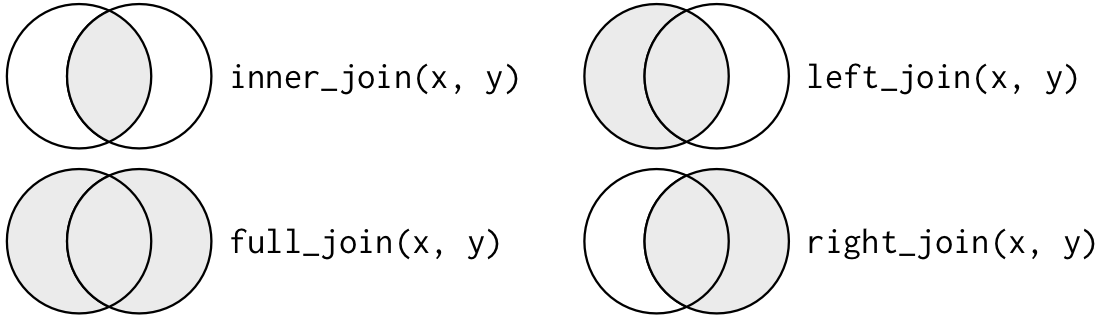
\includegraphics{_bookdown_files/presentation-intro_files/figure-html/join-venn.png}

\begin{Shaded}
\begin{Highlighting}[]
\NormalTok{flights }\OperatorTok\StringTok{ }
\StringTok{  }\KeywordTok{select}\NormalTok{(year}\OperatorTok{:}\NormalTok{day, hour, origin, dest, tailnum, carrier) }\OperatorTok\StringTok{ }
\StringTok{  }\KeywordTok{left_join}\NormalTok{(airlines, }\DataTypeTok{by =} \KeywordTok{c}\NormalTok{(}\StringTok{"carrier"}\NormalTok{ =}\StringTok{ "carrier"}\NormalTok{))}
\end{Highlighting}
\end{Shaded}

\begin{verbatim}
## # A tibble: 336,776 x 9
##     year month   day  hour origin dest  tailnum carrier name               
##    <int> <int> <int> <dbl> <chr>  <chr> <chr>   <chr>   <chr>              
##  1  2013     1     1     5 EWR    IAH   N14228  UA      United Air Lines I~
##  2  2013     1     1     5 LGA    IAH   N24211  UA      United Air Lines I~
##  3  2013     1     1     5 JFK    MIA   N619AA  AA      American Airlines ~
##  4  2013     1     1     5 JFK    BQN   N804JB  B6      JetBlue Airways    
##  5  2013     1     1     6 LGA    ATL   N668DN  DL      Delta Air Lines In~
##  6  2013     1     1     5 EWR    ORD   N39463  UA      United Air Lines I~
##  7  2013     1     1     6 EWR    FLL   N516JB  B6      JetBlue Airways    
##  8  2013     1     1     6 LGA    IAD   N829AS  EV      ExpressJet Airline~
##  9  2013     1     1     6 JFK    MCO   N593JB  B6      JetBlue Airways    
## 10  2013     1     1     6 LGA    ORD   N3ALAA  AA      American Airlines ~
## # ... with 336,766 more rows
\end{verbatim}

\hypertarget{excercise-9}{%
\section{Excercise 9}\label{excercise-9}}

\begin{itemize}
\tightlist
\item
  Left join your data with \texttt{tele2-kunder-transaktioner.csv} on \texttt{custid}.
\end{itemize}

\hypertarget{tidy-data}{%
\section{Tidy data}\label{tidy-data}}

\begin{itemize}
\tightlist
\item
  \texttt{tidy} data is when every observation is a row and every variable is a column.
\end{itemize}

\begin{Shaded}
\begin{Highlighting}[]
\KeywordTok{library}\NormalTok{(gapminder)}
\NormalTok{gapminder}
\end{Highlighting}
\end{Shaded}

\begin{verbatim}
## # A tibble: 1,704 x 6
##    country     continent  year lifeExp      pop gdpPercap
##    <fct>       <fct>     <int>   <dbl>    <int>     <dbl>
##  1 Afghanistan Asia       1952    28.8  8425333      779.
##  2 Afghanistan Asia       1957    30.3  9240934      821.
##  3 Afghanistan Asia       1962    32.0 10267083      853.
##  4 Afghanistan Asia       1967    34.0 11537966      836.
##  5 Afghanistan Asia       1972    36.1 13079460      740.
##  6 Afghanistan Asia       1977    38.4 14880372      786.
##  7 Afghanistan Asia       1982    39.9 12881816      978.
##  8 Afghanistan Asia       1987    40.8 13867957      852.
##  9 Afghanistan Asia       1992    41.7 16317921      649.
## 10 Afghanistan Asia       1997    41.8 22227415      635.
## # ... with 1,694 more rows
\end{verbatim}

\hypertarget{untidy-data}{%
\section{Untidy data}\label{untidy-data}}

\begin{Shaded}
\begin{Highlighting}[]
\KeywordTok{library}\NormalTok{(readxl)}
\NormalTok{gapminder_untidy <-}\StringTok{ }\KeywordTok{read_excel}\NormalTok{(}\StringTok{"_bookdown_files/data/life_expectancy_at_birth.xlsx"}\NormalTok{)}
\NormalTok{gapminder_untidy }
\end{Highlighting}
\end{Shaded}

\begin{verbatim}
## # A tibble: 260 x 218
##    `Life expectanc~ `1800` `1801` `1802` `1803` `1804` `1805` `1806` `1807`
##    <chr>             <dbl>  <dbl>  <dbl>  <dbl>  <dbl>  <dbl>  <dbl>  <dbl>
##  1 Abkhazia           NA     NA     NA     NA     NA     NA     NA     NA  
##  2 Afghanistan        28.2   28.2   28.2   28.2   28.2   28.2   28.2   28.1
##  3 Akrotiri and Dh~   NA     NA     NA     NA     NA     NA     NA     NA  
##  4 Albania            35.4   35.4   35.4   35.4   35.4   35.4   35.4   35.4
##  5 Algeria            28.8   28.8   28.8   28.8   28.8   28.8   28.8   28.8
##  6 American Samoa     NA     NA     NA     NA     NA     NA     NA     NA  
##  7 Andorra            NA     NA     NA     NA     NA     NA     NA     NA  
##  8 Angola             27.0   27.0   27.0   27.0   27.0   27.0   27.0   27.0
##  9 Anguilla           NA     NA     NA     NA     NA     NA     NA     NA  
## 10 Antigua and Bar~   33.5   33.5   33.5   33.5   33.5   33.5   33.5   33.5
## # ... with 250 more rows, and 209 more variables: `1808` <dbl>,
## #   `1809` <dbl>, `1810` <dbl>, `1811` <dbl>, `1812` <dbl>, `1813` <dbl>,
## #   `1814` <dbl>, `1815` <dbl>, `1816` <dbl>, `1817` <dbl>, `1818` <dbl>,
## #   `1819` <dbl>, `1820` <dbl>, `1821` <dbl>, `1822` <dbl>, `1823` <dbl>,
## #   `1824` <dbl>, `1825` <dbl>, `1826` <dbl>, `1827` <dbl>, `1828` <dbl>,
## #   `1829` <dbl>, `1830` <dbl>, `1831` <dbl>, `1832` <dbl>, `1833` <dbl>,
## #   `1834` <dbl>, `1835` <dbl>, `1836` <dbl>, `1837` <dbl>, `1838` <dbl>,
## #   `1839` <dbl>, `1840` <dbl>, `1841` <dbl>, `1842` <dbl>, `1843` <dbl>,
## #   `1844` <dbl>, `1845` <dbl>, `1846` <dbl>, `1847` <dbl>, `1848` <dbl>,
## #   `1849` <dbl>, `1850` <dbl>, `1851` <dbl>, `1852` <dbl>, `1853` <dbl>,
## #   `1854` <dbl>, `1855` <dbl>, `1856` <dbl>, `1857` <dbl>, `1858` <dbl>,
## #   `1859` <dbl>, `1860` <dbl>, `1861` <dbl>, `1862` <dbl>, `1863` <dbl>,
## #   `1864` <dbl>, `1865` <dbl>, `1866` <dbl>, `1867` <dbl>, `1868` <dbl>,
## #   `1869` <dbl>, `1870` <dbl>, `1871` <dbl>, `1872` <dbl>, `1873` <dbl>,
## #   `1874` <dbl>, `1875` <dbl>, `1876` <dbl>, `1877` <dbl>, `1878` <dbl>,
## #   `1879` <dbl>, `1880` <dbl>, `1881` <dbl>, `1882` <dbl>, `1883` <dbl>,
## #   `1884` <dbl>, `1885` <dbl>, `1886` <dbl>, `1887` <dbl>, `1888` <dbl>,
## #   `1889` <dbl>, `1890` <dbl>, `1891` <dbl>, `1892` <dbl>, `1893` <dbl>,
## #   `1894` <dbl>, `1895` <dbl>, `1896` <dbl>, `1897` <dbl>, `1898` <dbl>,
## #   `1899` <dbl>, `1900` <dbl>, `1901` <dbl>, `1902` <dbl>, `1903` <dbl>,
## #   `1904` <dbl>, `1905` <dbl>, `1906` <dbl>, `1907` <dbl>, ...
\end{verbatim}

We want to gather the columns

\begin{Shaded}
\begin{Highlighting}[]
\NormalTok{data }\OperatorTok\StringTok{ }
\StringTok{  }\KeywordTok{gather}\NormalTok{(key, value, columns_to_gather)}
\end{Highlighting}
\end{Shaded}

\begin{Shaded}
\begin{Highlighting}[]
\NormalTok{gapminder_untidy }\OperatorTok\StringTok{ }
\StringTok{  }\KeywordTok{gather}\NormalTok{(}\DataTypeTok{key =}\NormalTok{ year, }\DataTypeTok{value =}\NormalTok{ life_expectancy, }\OperatorTok{-}\StringTok{`}\DataTypeTok{Life expectancy}\StringTok{`}\NormalTok{) }\OperatorTok
\StringTok{  }\KeywordTok{rename}\NormalTok{(}\DataTypeTok{land =} \StringTok{`}\DataTypeTok{Life expectancy}\StringTok{`}\NormalTok{) }\OperatorTok\StringTok{ }
\StringTok{  }\KeywordTok{mutate}\NormalTok{(}\DataTypeTok{life_expectancy =} \KeywordTok{as.numeric}\NormalTok{(life_expectancy))}
\end{Highlighting}
\end{Shaded}

\begin{verbatim}
## # A tibble: 56,420 x 3
##    land                  year  life_expectancy
##    <chr>                 <chr>           <dbl>
##  1 Abkhazia              1800             NA  
##  2 Afghanistan           1800             28.2
##  3 Akrotiri and Dhekelia 1800             NA  
##  4 Albania               1800             35.4
##  5 Algeria               1800             28.8
##  6 American Samoa        1800             NA  
##  7 Andorra               1800             NA  
##  8 Angola                1800             27.0
##  9 Anguilla              1800             NA  
## 10 Antigua and Barbuda   1800             33.5
## # ... with 56,410 more rows
\end{verbatim}

\begin{itemize}
\tightlist
\item
  \texttt{spread()} does the opposite.
\end{itemize}

\hypertarget{excercise-10}{%
\section{Excercise 10}\label{excercise-10}}

\begin{itemize}
\item
  In your data set you have 12 columns for data volume consumption per month, \texttt{tr\_tot\_data\_vol\_all\_netw\_1:tr\_tot\_data\_vol\_all\_netw\_12}
\item
  Every column represent a month and you want to calculate the mean of data volume consumption over time.
\item
  The columns represent a month
\item
  The first column \texttt{tr\_tot\_data\_vol\_all\_netw\_1} is the latest month, i.e. ``2019-04-30''
\item
  Create a vector with all the month dates corresponding to the columns.
\item
  R function called \texttt{seq()}
\end{itemize}

\begin{Shaded}
\begin{Highlighting}[]
\NormalTok{new_cols <-}\StringTok{ }\KeywordTok{seq}\NormalTok{(}\DataTypeTok{from =} \KeywordTok{as.Date}\NormalTok{(}\StringTok{"2018-05-30"}\NormalTok{), }\DataTypeTok{by =} \StringTok{"month"}\NormalTok{, }\DataTypeTok{length.out =} \DecValTok{12}\NormalTok{) }\OperatorTok\StringTok{ }
\StringTok{  }\KeywordTok{as.character}\NormalTok{()}

\NormalTok{new_cols}
\end{Highlighting}
\end{Shaded}

\begin{verbatim}
##  [1] "2018-05-30" "2018-06-30" "2018-07-30" "2018-08-30" "2018-09-30"
##  [6] "2018-10-30" "2018-11-30" "2018-12-30" "2019-01-30" "2019-03-02"
## [11] "2019-03-30" "2019-04-30"
\end{verbatim}

Rename every column by it's date.

\begin{Shaded}
\begin{Highlighting}[]
\NormalTok{kunder }\OperatorTok\StringTok{ }
\StringTok{  }\KeywordTok{select}\NormalTok{(cust_id, source_date, pc_priceplan_nm, tr_tot_data_vol_all_netw_}\DecValTok{1}\OperatorTok{:}\NormalTok{tr_tot_data_vol_all_netw_}\DecValTok{12}\NormalTok{) }\OperatorTok\StringTok{ }
\StringTok{  }\KeywordTok{rename_at}\NormalTok{(}\KeywordTok{vars}\NormalTok{(tr_tot_data_vol_all_netw_}\DecValTok{1}\OperatorTok{:}\NormalTok{tr_tot_data_vol_all_netw_}\DecValTok{12}\NormalTok{), }\OperatorTok{~}\NormalTok{new_cols)}
\end{Highlighting}
\end{Shaded}

\begin{itemize}
\tightlist
\item
  Fill in the \texttt{sort(decreasing\ =\ )} to \texttt{TRUE}
\item
  Gather the data into two new columns called \texttt{data\_month} and \texttt{data\_volume}
\item
  Turn \texttt{data\_month} into a date-column
\end{itemize}

\begin{Shaded}
\begin{Highlighting}[]
\NormalTok{new_cols <-}\StringTok{ }\KeywordTok{seq}\NormalTok{(}\DataTypeTok{from =} \KeywordTok{as.Date}\NormalTok{(}\StringTok{"2018-05-30"}\NormalTok{), }\DataTypeTok{by =} \StringTok{"month"}\NormalTok{, }\DataTypeTok{length.out =} \DecValTok{12}\NormalTok{) }\OperatorTok\StringTok{ }
\StringTok{  }\KeywordTok{sort}\NormalTok{(}\DataTypeTok{decreasing =}\NormalTok{ ) }\OperatorTok\StringTok{ }
\StringTok{  }\KeywordTok{as.character}\NormalTok{() }

\NormalTok{kunder_tidy_month <-}\StringTok{ }\NormalTok{kunder }\OperatorTok\StringTok{ }
\StringTok{  }\KeywordTok{select}\NormalTok{(cust_id, source_date, pc_priceplan_nm, tr_tot_data_vol_all_netw_}\DecValTok{1}\OperatorTok{:}\NormalTok{tr_tot_data_vol_all_netw_}\DecValTok{12}\NormalTok{) }\OperatorTok\StringTok{ }
\StringTok{  }\KeywordTok{rename_at}\NormalTok{(}\KeywordTok{vars}\NormalTok{(tr_tot_data_vol_all_netw_}\DecValTok{1}\OperatorTok{:}\NormalTok{tr_tot_data_vol_all_netw_}\DecValTok{12}\NormalTok{), }\OperatorTok{~}\NormalTok{new_cols) }\OperatorTok\StringTok{ }
\StringTok{  }\KeywordTok{gather}\NormalTok{(... , ... , }\StringTok{`}\DataTypeTok{2018-05-30}\StringTok{`}\OperatorTok{:}\StringTok{`}\DataTypeTok{2019-04-30}\StringTok{`}\NormalTok{) }\OperatorTok\StringTok{ }
\StringTok{  }\KeywordTok{mutate}\NormalTok{(}\DataTypeTok{data_month =} \KeywordTok{as.Date}\NormalTok{(data_month))}
\end{Highlighting}
\end{Shaded}

\begin{itemize}
\tightlist
\item
  Calculate the mean value per priceplan and month
\end{itemize}

\begin{Shaded}
\begin{Highlighting}[]
\NormalTok{mean_volume_sum <-}\StringTok{ }\NormalTok{kunder_tidy_month }\OperatorTok\StringTok{ }
\StringTok{  }\KeywordTok{group_by}\NormalTok{(pc_priceplan_nm, data_month) }\OperatorTok\StringTok{ }
\StringTok{  }\KeywordTok{summarise}\NormalTok{(}\DataTypeTok{mean_volume =} \KeywordTok{mean}\NormalTok{(data_volume, }\DataTypeTok{na.rm =}\NormalTok{ T))}

\NormalTok{mean_volume_sum }
\end{Highlighting}
\end{Shaded}

Execute the code to visualize:

\begin{Shaded}
\begin{Highlighting}[]
\NormalTok{p <-}\StringTok{ }\KeywordTok{ggplot}\NormalTok{(mean_volume_sum, }
         \KeywordTok{aes}\NormalTok{(}\DataTypeTok{x =}\NormalTok{ data_month, }\DataTypeTok{y =}\NormalTok{ mean_volume, }\DataTypeTok{color =}\NormalTok{ pc_priceplan_nm)) }\OperatorTok{+}
\StringTok{  }\KeywordTok{geom_line}\NormalTok{() }\OperatorTok{+}
\StringTok{  }\KeywordTok{scale_color_discrete}\NormalTok{() }\OperatorTok{+}
\StringTok{  }\KeywordTok{theme}\NormalTok{(}\DataTypeTok{legend.position =} \StringTok{"none"}\NormalTok{)}
\end{Highlighting}
\end{Shaded}

\begin{Shaded}
\begin{Highlighting}[]
\NormalTok{widget <-}\StringTok{ }\NormalTok{plotly}\OperatorTok{::}\KeywordTok{ggplotly}\NormalTok{(p)}
\NormalTok{htmlwidgets}\OperatorTok{::}\KeywordTok{saveWidget}\NormalTok{(widget, }\StringTok{"plotly_ex.html"}\NormalTok{)}
\end{Highlighting}
\end{Shaded}

\textless{}iframe src=``plotly\_ex.html'' width = ``900px'', height = ``600px'' frameBorder=``0''\textgreater{}

\hypertarget{methods}{%
\chapter{Methods}\label{methods}}

We describe our methods in this chapter.

\hypertarget{applications}{%
\chapter{Applications}\label{applications}}

Some \emph{significant} applications are demonstrated in this chapter.

\hypertarget{example-one}{%
\section{Example one}\label{example-one}}

\hypertarget{example-two}{%
\section{Example two}\label{example-two}}

\hypertarget{final-words}{%
\chapter{Final Words}\label{final-words}}

We have finished a nice book.

\bibliography{book.bib,packages.bib}


\end{document}
